\chapter{Ethical Analysis}

\section{Ethical Justification}
The basis for this project is that all students should be able to receive help from others. However it can be difficult for certain student groups to set up meetings with others. For example, it can be inconvenient for commuters to meet up without prior planning. The purpose of our project is to allow students to easily collaborate with one another. We hope that this application will allow students to help one another either by using it to communicate with one another or organize meetings.

The following table includes principles from the Software Engineering Code of Ethics that apply to the justification of our project:

\begin{figure}[h]
	\centering
	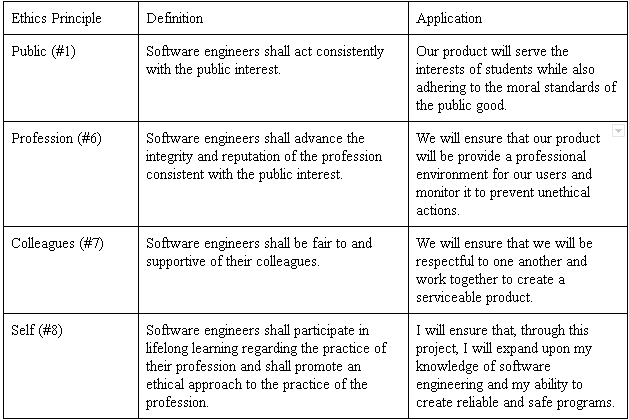
\includegraphics[scale=0.8]{images/ethics_table.png}
	\caption{Ethics Table}
	\label{fig:ethics table}
\end{figure}

\section{Organization}
Our project takes into consideration the availability of the web and how many devices are able to access it. We are aware that its availability will allow students to easily contact each other. Because of the availability of the internet, we want to encourage students to help each other succeed. We are also aware that this gives many different people access to our application and that it requires some sort of monitoring. 

In regards to our team, we realize that we need to work together in order to be more efficient. We are committed to having good communication so that we know that what we do is ethical and beneficial to our product.

\section{Effects on Society and Culture}
As with any platform that involves communication through the web, we need to be aware of the issue of cyberbullying. Because of application will provide a means for students to communicate with each other, it is also possible that users of malicious intent will harass others. Therefore, it is our duty to maintain a safe and friendly environment and ensure that our customers are free from any type of harassment.

Another ethical issue our product may come across is plagiarism or cheating. Because we want to create a platform where students can communicate with each other, this also allow them to share notes and other work. While we do believe this can be useful for student learning, it can also lead to cheating and/or plagiarism. I believe responsibility for this falls to both the product creators (my partner and me) and the user. The best my partner and I can do is limit the type of data that can be shared through our application. For example, we could restrict files or have a moderator (but that may prove to be difficult). However, it is also up to the users to avoid posting or copying the information that is shared.